\section{The particle filter as an interacting particle system}
\label{sec:pf_interacting}

The particle filter is not only an approximation to one posterior; it is a stochastic process whose time marginals converge, as the number of particles grows, to the predictive laws of the model, and whose reweighted particle clouds converge to the sequence of filtering posteriors. We use the notation of Section~\ref{sec:pf_errors}. Define, for each probability measure $\eta$, the McKean kernel $K_{t,\eta}(x,\cdot) = \Psi_t(\eta)M$, which does not depend on $x$ but depends on $\eta$: a particle at $x$ is replaced by a draw from the updated law and then moved. This is a nonlinear Markov chain in the sense of McKean, the discrete time analogue of the McKean Vlasov processes of Chapter~\ref{ch:kinetic}.

\begin{proposition}[The marginals are the posteriors]
\label{prop:pf_marginals}
Let $\bar X_1\sim\eta_1$ and, recursively, $\bar X_{t+1}\mid\bar X_t\sim K_{t,\mathrm{Law}(\bar X_t)}(\bar X_t,\cdot)$. Then $\mathrm{Law}(\bar X_t) = \eta_t$ for every $t$, and $\Psi_t(\mathrm{Law}(\bar X_t)) = \pi_t$. The time marginals of the nonlinear chain are therefore the predictive laws, and their Bayes updates are the filtering posteriors.
\end{proposition}

\begin{proof}
By induction. If $\mathrm{Law}(\bar X_t) = \eta_t$, then $\mathrm{Law}(\bar X_{t+1}) = \int\eta_t(\dd x)K_{t,\eta_t}(x,\cdot) = \Psi_t(\eta_t)M = \pi_tM = \eta_{t+1}$, and $\Psi_t(\eta_t) = \pi_t$ by Bayes' rule.
\end{proof}

Only the time marginals are asserted. The kernel $K_{t,\eta}(x,\cdot)$ does not depend on $x$, so the values $\bar X_1,\bar X_2,\dots$ are independent, and the law of the path of the chain is the product of the $\eta_t$, not a posterior for the path of the hidden state.

The bootstrap filter is the $N$ particle mean field approximation of this chain: each particle moves by $K_{t,\eta^N_t}$ with the unknown law replaced by the empirical measure $\eta^N_t$. Under the hypotheses of Theorem~\ref{thm:pf_error}, $\eta^N_t$ converges to the deterministic limit $\eta_t$. The particles are exchangeable, so Theorem~\ref{thm:sznitman} shows that the law of each particle at time $t$ converges to $\eta_t$ and that any $k$ particles become independent: the bootstrap filter propagates chaos. A single forward pass with $N$ particles, at cost $O(NT)$, thus delivers approximations to every intermediate posterior $p(x_t\mid y_{1:t})$, $t = 1,\dots,T$, not just the last one (upper panel of Figure~\ref{fig:pl}). Markov chain Monte Carlo, by contrast, targets one posterior at a time and must be rerun when a new observation arrives.

The resampling step selects, for each new particle, an ancestor index $a^i_t\in\{1,\dots,N\}$. These indices are discrete latent variables that switch at every step, and conditionally on the whole ancestry the particles move independently. The particle system is therefore itself a switching model on an extended space, with the ancestor indices as regimes; Andrieu, Doucet and Holenstein used this extended space construction to prove the exactness of particle Markov chain Monte Carlo~\cite{adh2010}. In continuous time the switching structure can be made part of the model itself (Section~\ref{sec:kurtz_xiong}). When the only latent state is a finite regime and the observation densities given the regime are known, the filter is exact and finite dimensional, Hamilton's filter~\cite{hamilton1989}, which is the forward algorithm for hidden Markov models of Section~\ref{sec:wonham}. When the state is linear and Gaussian given the path of the regime, each particle can carry the regime together with the Kalman mean and variance of the continuous state instead of a sampled value. This is the mixture Kalman filter of Chen and Liu~\cite{chenliu2000}, and by the Rao Blackwell inequality $\Var(\E[f\mid s])\leq\Var(f)$ it reduces the variance of the importance weights~\cite{dga2000}. The general principle is that a particle should carry the smallest summary of the past that makes the future conditionally tractable.

\section{Particle learning and conditional sufficient statistics}
\label{sec:particle_learning}

The principle applies to static parameters, where the naive particle filter fails. Suppose the model has parameter $\theta$ and that there are conditional sufficient statistics $s_t$, updated deterministically by
\[
s_{t+1} = S(s_t,x_t,x_{t+1},y_{t+1}),
\]
such that $p(\theta\mid x_{0:t},y_{1:t}) = p(\theta\mid s_t)$. This is the case in conditionally conjugate models, where the posterior of $\theta$ given the states and the data lies in a conjugate family with a sufficient statistic of fixed dimension. An example is the linear Gaussian state space model with unknown variances, treated below. Particle learning, introduced by Carvalho, Johannes, Lopes and Polson~\cite{cjlp2010}, tracks the essential state $z_t = (x_t,s_t,\theta)$ and updates it in a resample and propagate order:
\begin{enumerate}
\item Resample $\{z^i_t\}$ with weights proportional to the predictive likelihood $p(y_{t+1}\mid z^i_t) = \int p(y_{t+1}\mid x_{t+1},\theta)\,p(x_{t+1}\mid x_t,\theta)\dd x_{t+1}$.
\item Propagate $x^i_{t+1}\sim p(x_{t+1}\mid z^i_t,y_{t+1})$.
\item Update the sufficient statistics $s^i_{t+1} = S(s^i_t,x^i_t,x^i_{t+1},y_{t+1})$.
\item Draw $\theta^i\sim p(\theta\mid s^i_{t+1})$.
\end{enumerate}

\begin{proposition}[Exactness of the particle learning step]
\label{prop:pl_exact}
Let $z_t$ have the law $p(z_t\mid y_{1:t})$. Reweight this law by the predictive likelihood $p(y_{t+1}\mid z_t)$, which is step one at the level of laws, and then apply steps two to four. The new essential state $(x_{t+1},s_{t+1},\theta)$ has the law $p(x_{t+1},s_{t+1},\theta\mid y_{1:t+1})$.
\end{proposition}

\begin{proof}
By Bayes' rule, the reweighted law is $p(z_t\mid y_{1:t+1})\propto p(y_{t+1}\mid z_t)\,p(z_t\mid y_{1:t})$, since $y_{t+1}$ depends on the past only through $z_t$, and $p(x_{t+1}\mid z_t,y_{1:t+1}) = p(x_{t+1}\mid z_t,y_{t+1})$ by the Markov structure, which is step two. Hence after step two $(z_t,x_{t+1})$ has the law $p(z_t,x_{t+1}\mid y_{1:t+1})$, and $s_{t+1}$ is a deterministic function of it. It remains to show that $\theta$ redrawn in step four has the correct conditional law given $(x_{t+1},s_{t+1})$. Conditionally on the whole path $(x_{0:t+1},y_{1:t+1})$ the posterior of $\theta$ is $p(\theta\mid s_{t+1})$ by sufficiency. Since this depends on the path only through $s_{t+1}$, it is also the conditional law of $\theta$ given $(x_{t+1},s_{t+1},y_{1:t+1})$, by the tower property. Drawing $\theta$ afresh from it therefore leaves the joint law of $(x_{t+1},s_{t+1},\theta)$ equal to the posterior.
\end{proof}

The $N$ particle algorithm replaces the laws by empirical measures and the reweighting of step one by multinomial resampling, so it is an interacting particle approximation of this exact recursion. Two features distinguish particle learning from the naive filter. First, resampling uses the predictive likelihood before propagation, as in the auxiliary particle filter of Pitt and Shephard~\cite{pittshephard1999}, so particles are moved into regions supported by the new observation instead of being proposed blindly and then killed. Second, the parameter is redrawn at every step from its conditional posterior. The parameter cloud is therefore regenerated rather than inherited, and its values do not collapse onto the few distinct values that destroy the naive filter. What is inherited is the sufficient statistic, a deterministic function of the particle's path. It is subject to the path degeneracy of Section~\ref{sec:pf_errors}: particles that share an ancestor share the part of $s_t$ accumulated along the ancestral path. The essential state is also not mixing, since $s_t$ is a running sum and $\theta$ is static, so Theorem~\ref{thm:pf_error} gives no bound uniform in time for particle learning, and the Monte Carlo error of the parameter posterior can accumulate over long horizons. Chopin and coauthors~\cite{chopin2010} raised the potential for degeneracy in particle learning, related to the exponential forgetting of the past simulations, in their discussion of the method, while Carvalho, Johannes, Lopes and Polson~\cite{cjlp2010} report in simulations that the method is robust to degeneracy as the sample size grows.

\begin{example}[Local level model with unknown variances]
\label{ex:pl_local_level}
Let $x_t = x_{t-1}+\sqrt q\,\varepsilon_t$ and $y_t = x_t+\sqrt r\,\nu_t$, where $\varepsilon_t$ and $\nu_t$ are independent standard normal and $x_0\sim N(0,4)$, and let $q$ and $r$ have independent inverse Gamma priors $\mathrm{IG}(a_0,b_0)$, with density proportional to $\tau^{-a_0-1}e^{-b_0/\tau}$. The essential state is $z_t = (x_t,s^q_t,s^r_t,q,r)$ with sufficient statistics
\[
s^q_t = \sum_{u=1}^t(x_u-x_{u-1})^2,\qquad s^r_t = \sum_{u=1}^t(y_u-x_u)^2,
\]
and conditional posteriors $q\mid s_t\sim\mathrm{IG}(a_0+\frac t2,b_0+\frac12s^q_t)$ and $r\mid s_t\sim\mathrm{IG}(a_0+\frac t2,b_0+\frac12s^r_t)$. The predictive likelihood is $p(y_{t+1}\mid z_t) = N(y_{t+1};x_t,q+r)$, and the propagation density is Gaussian with variance $v = (q^{-1}+r^{-1})^{-1}$ and mean $v(x_t/q+y_{t+1}/r)$. Step one resamples with these explicit weights, and steps two to four are exact draws from known distributions.
\end{example}

Figure~\ref{fig:pl} applies particle learning with $N = 5000$ particles to $T = 400$ observations simulated with $q = 0.25$ and $r = 1$, with priors $\mathrm{IG}(3,1)$. The lower panels show the posterior medians and $90\%$ bands of $q$ and $r$ as functions of $t$, every one of which is a by product of the same run. They concentrate around the true values, with final medians $0.29$ and $1.01$. For comparison, a naive bootstrap filter with the same number of particles and the same data, which carries $(x_t,q,r)$ with the parameters fixed at their prior draws, ends with only three distinct values of $q$.

\begin{figure}[t]
\centering
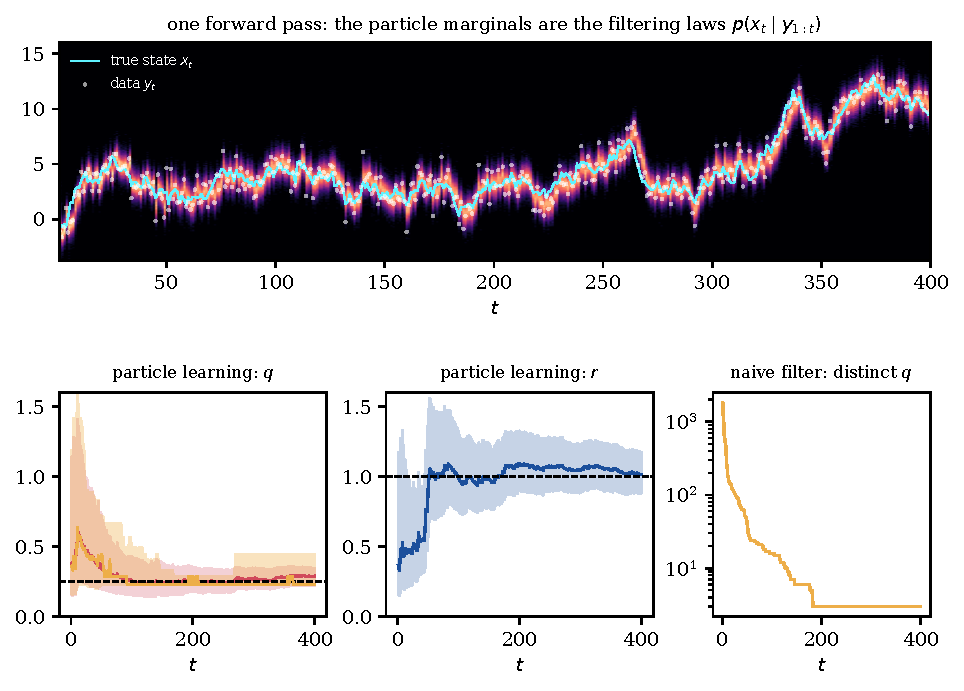
\includegraphics[width=\textwidth]{particle_learning}
\caption{Particle learning with $N = 5000$ particles for the local level model with unknown variances. Top, the particle histograms at each time from one forward pass, which are the filtering laws $p(x_t\mid y_{1:t})$, with the true state and the data. Bottom left and middle, sequential posterior medians and $90\%$ bands for $q$ and $r$, with the true values dashed; the lighter median and band at left are those of the naive filter for $q$. Bottom right, on a logarithmic scale, the number of distinct values of $q$ in the naive filter, which collapses to three.}
\label{fig:pl}
\end{figure}

Carvalho, Johannes, Lopes and Polson~\cite{cjlp2010} extend particle learning to smoothing by backward resampling, in the manner of Godsill, Doucet and West~\cite{gdw2004}, and to sequential model comparison through the predictive likelihoods computed in step one, whose running product is a particle estimate of the marginal likelihood. Carvalho, Lopes, Polson and Taddy~\cite{clpt2010} extend it to general mixtures and nonparametric mixtures. Its precursors are the sufficient statistic filters of Storvik~\cite{storvik2002} and Fearnhead~\cite{fearnhead2002}. In the language of this book, particle learning applies to filtering the lesson of the moment conditioning chapter, Chapter~\ref{ch:types}: carry the conditional sufficient statistics, the macroscopic variables, and let the remaining randomness be regenerated from its exact conditional law. In the language of de Finetti, when the observations are conditionally independent given $\theta$ the conditional sufficient statistic is the summary of the past through which the mixing variable $\theta$ is learned, and the particle carries the same summary in the presence of hidden states.
